\PassOptionsToPackage{unicode=true}{hyperref} % options for packages loaded elsewhere
\PassOptionsToPackage{hyphens}{url}
%
\documentclass[]{article}
\usepackage{lmodern}
\usepackage{amssymb,amsmath}
\usepackage{ifxetex,ifluatex}
\usepackage{fixltx2e} % provides \textsubscript
\ifnum 0\ifxetex 1\fi\ifluatex 1\fi=0 % if pdftex
  \usepackage[T1]{fontenc}
  \usepackage[utf8]{inputenc}
  \usepackage{textcomp} % provides euro and other symbols
\else % if luatex or xelatex
  \usepackage{unicode-math}
  \defaultfontfeatures{Ligatures=TeX,Scale=MatchLowercase}
\fi
% use upquote if available, for straight quotes in verbatim environments
\IfFileExists{upquote.sty}{\usepackage{upquote}}{}
% use microtype if available
\IfFileExists{microtype.sty}{%
\usepackage[]{microtype}
\UseMicrotypeSet[protrusion]{basicmath} % disable protrusion for tt fonts
}{}
\IfFileExists{parskip.sty}{%
\usepackage{parskip}
}{% else
\setlength{\parindent}{0pt}
\setlength{\parskip}{6pt plus 2pt minus 1pt}
}
\usepackage{hyperref}
\hypersetup{
            pdftitle={BiasVarianceTradeoff.rmd},
            pdfauthor={Shan Chen},
            pdfborder={0 0 0},
            breaklinks=true}
\urlstyle{same}  % don't use monospace font for urls
\usepackage[margin=1in]{geometry}
\usepackage{color}
\usepackage{fancyvrb}
\newcommand{\VerbBar}{|}
\newcommand{\VERB}{\Verb[commandchars=\\\{\}]}
\DefineVerbatimEnvironment{Highlighting}{Verbatim}{commandchars=\\\{\}}
% Add ',fontsize=\small' for more characters per line
\usepackage{framed}
\definecolor{shadecolor}{RGB}{248,248,248}
\newenvironment{Shaded}{\begin{snugshade}}{\end{snugshade}}
\newcommand{\AlertTok}[1]{\textcolor[rgb]{0.94,0.16,0.16}{#1}}
\newcommand{\AnnotationTok}[1]{\textcolor[rgb]{0.56,0.35,0.01}{\textbf{\textit{#1}}}}
\newcommand{\AttributeTok}[1]{\textcolor[rgb]{0.77,0.63,0.00}{#1}}
\newcommand{\BaseNTok}[1]{\textcolor[rgb]{0.00,0.00,0.81}{#1}}
\newcommand{\BuiltInTok}[1]{#1}
\newcommand{\CharTok}[1]{\textcolor[rgb]{0.31,0.60,0.02}{#1}}
\newcommand{\CommentTok}[1]{\textcolor[rgb]{0.56,0.35,0.01}{\textit{#1}}}
\newcommand{\CommentVarTok}[1]{\textcolor[rgb]{0.56,0.35,0.01}{\textbf{\textit{#1}}}}
\newcommand{\ConstantTok}[1]{\textcolor[rgb]{0.00,0.00,0.00}{#1}}
\newcommand{\ControlFlowTok}[1]{\textcolor[rgb]{0.13,0.29,0.53}{\textbf{#1}}}
\newcommand{\DataTypeTok}[1]{\textcolor[rgb]{0.13,0.29,0.53}{#1}}
\newcommand{\DecValTok}[1]{\textcolor[rgb]{0.00,0.00,0.81}{#1}}
\newcommand{\DocumentationTok}[1]{\textcolor[rgb]{0.56,0.35,0.01}{\textbf{\textit{#1}}}}
\newcommand{\ErrorTok}[1]{\textcolor[rgb]{0.64,0.00,0.00}{\textbf{#1}}}
\newcommand{\ExtensionTok}[1]{#1}
\newcommand{\FloatTok}[1]{\textcolor[rgb]{0.00,0.00,0.81}{#1}}
\newcommand{\FunctionTok}[1]{\textcolor[rgb]{0.00,0.00,0.00}{#1}}
\newcommand{\ImportTok}[1]{#1}
\newcommand{\InformationTok}[1]{\textcolor[rgb]{0.56,0.35,0.01}{\textbf{\textit{#1}}}}
\newcommand{\KeywordTok}[1]{\textcolor[rgb]{0.13,0.29,0.53}{\textbf{#1}}}
\newcommand{\NormalTok}[1]{#1}
\newcommand{\OperatorTok}[1]{\textcolor[rgb]{0.81,0.36,0.00}{\textbf{#1}}}
\newcommand{\OtherTok}[1]{\textcolor[rgb]{0.56,0.35,0.01}{#1}}
\newcommand{\PreprocessorTok}[1]{\textcolor[rgb]{0.56,0.35,0.01}{\textit{#1}}}
\newcommand{\RegionMarkerTok}[1]{#1}
\newcommand{\SpecialCharTok}[1]{\textcolor[rgb]{0.00,0.00,0.00}{#1}}
\newcommand{\SpecialStringTok}[1]{\textcolor[rgb]{0.31,0.60,0.02}{#1}}
\newcommand{\StringTok}[1]{\textcolor[rgb]{0.31,0.60,0.02}{#1}}
\newcommand{\VariableTok}[1]{\textcolor[rgb]{0.00,0.00,0.00}{#1}}
\newcommand{\VerbatimStringTok}[1]{\textcolor[rgb]{0.31,0.60,0.02}{#1}}
\newcommand{\WarningTok}[1]{\textcolor[rgb]{0.56,0.35,0.01}{\textbf{\textit{#1}}}}
\usepackage{graphicx,grffile}
\makeatletter
\def\maxwidth{\ifdim\Gin@nat@width>\linewidth\linewidth\else\Gin@nat@width\fi}
\def\maxheight{\ifdim\Gin@nat@height>\textheight\textheight\else\Gin@nat@height\fi}
\makeatother
% Scale images if necessary, so that they will not overflow the page
% margins by default, and it is still possible to overwrite the defaults
% using explicit options in \includegraphics[width, height, ...]{}
\setkeys{Gin}{width=\maxwidth,height=\maxheight,keepaspectratio}
\setlength{\emergencystretch}{3em}  % prevent overfull lines
\providecommand{\tightlist}{%
  \setlength{\itemsep}{0pt}\setlength{\parskip}{0pt}}
\setcounter{secnumdepth}{0}
% Redefines (sub)paragraphs to behave more like sections
\ifx\paragraph\undefined\else
\let\oldparagraph\paragraph
\renewcommand{\paragraph}[1]{\oldparagraph{#1}\mbox{}}
\fi
\ifx\subparagraph\undefined\else
\let\oldsubparagraph\subparagraph
\renewcommand{\subparagraph}[1]{\oldsubparagraph{#1}\mbox{}}
\fi

% set default figure placement to htbp
\makeatletter
\def\fps@figure{htbp}
\makeatother


\title{BiasVarianceTradeoff.rmd}
\author{Shan Chen}
\date{2/16/2020}

\begin{document}
\maketitle

\hypertarget{assignments}{%
\section{Assignments}\label{assignments}}

\hypertarget{assignment-1}{%
\subsection{Assignment 1}\label{assignment-1}}

\begin{Shaded}
\begin{Highlighting}[]
\NormalTok{f1 <-}\StringTok{ }\ControlFlowTok{function}\NormalTok{(x) x}\OperatorTok{+}\DecValTok{2}
\NormalTok{f2 <-}\StringTok{ }\ControlFlowTok{function}\NormalTok{(x) (x}\DecValTok{-1}\NormalTok{)}\OperatorTok{*}\NormalTok{(x}\OperatorTok{+}\DecValTok{1}\NormalTok{)}
\NormalTok{f3 <-}\StringTok{ }\ControlFlowTok{function}\NormalTok{(x) x}\OperatorTok{*}\NormalTok{(x}\DecValTok{-1}\NormalTok{)}\OperatorTok{*}\NormalTok{(x}\OperatorTok{+}\DecValTok{1}\NormalTok{)}
\NormalTok{f4 <-}\StringTok{ }\ControlFlowTok{function}\NormalTok{(x) (x}\DecValTok{-1}\NormalTok{)}\OperatorTok{*}\NormalTok{(x}\OperatorTok{+}\DecValTok{1}\NormalTok{)}\OperatorTok{*}\NormalTok{(x}\DecValTok{-1}\NormalTok{)}\OperatorTok{*}\NormalTok{(x}\OperatorTok{+}\DecValTok{1}\NormalTok{)}
\end{Highlighting}
\end{Shaded}

Constuct data and dataframe

\begin{Shaded}
\begin{Highlighting}[]
\NormalTok{K <-}\StringTok{ }\DecValTok{101}
\CommentTok{## Range}
\NormalTok{xMin <-}\StringTok{ }\DecValTok{-1}
\NormalTok{xMax <-}\StringTok{ }\DecValTok{1}
\NormalTok{xVals<-}\KeywordTok{seq}\NormalTok{(xMin, xMax,}\DataTypeTok{length=}\NormalTok{K)}
\NormalTok{sizeDS <-}\DecValTok{50} \CommentTok{# number of data points}
\NormalTok{sig <-}\FloatTok{1.75} \CommentTok{# for the noise}
\NormalTok{buildData <-}\StringTok{ }\ControlFlowTok{function}\NormalTok{(f,sizeDS,sig,}\DataTypeTok{xMin =} \DecValTok{-1}\NormalTok{, }\DataTypeTok{xMax =} \DecValTok{1}\NormalTok{)\{}
\CommentTok{##predictor}
\NormalTok{x<-}\KeywordTok{runif}\NormalTok{(sizeDS,xMin, xMax) }\CommentTok{# inputs}
\CommentTok{## Repsonse}
\NormalTok{y<-}\KeywordTok{f}\NormalTok{(x)}\OperatorTok{+}\KeywordTok{rnorm}\NormalTok{(sizeDS,}\DecValTok{0}\NormalTok{,sig) }\CommentTok{#realized values f(x)+noise}
\CommentTok{## Put in a data frame}
\KeywordTok{data.frame}\NormalTok{(x,y)}
\NormalTok{\}}
\end{Highlighting}
\end{Shaded}

\begin{Shaded}
\begin{Highlighting}[]
\NormalTok{biasVarTO3 <-}\StringTok{ }\ControlFlowTok{function}\NormalTok{(form,sizeDS,numDS,x0)\{}
\NormalTok{  allVals <-}\StringTok{ }\KeywordTok{matrix}\NormalTok{(}\DataTypeTok{ncol=}\DecValTok{2}\NormalTok{,}\DataTypeTok{nrow=}\NormalTok{numDS)}
  \ControlFlowTok{for}\NormalTok{(m }\ControlFlowTok{in} \DecValTok{1}\OperatorTok{:}\NormalTok{numDS)\{}
\NormalTok{    mod <-}\StringTok{ }\KeywordTok{lm}\NormalTok{(}\KeywordTok{formula}\NormalTok{(form),}\KeywordTok{buildData}\NormalTok{(f,sizeDS,sig))}
\NormalTok{    pred <-}\StringTok{ }\KeywordTok{predict}\NormalTok{(mod,}\DataTypeTok{newdata=}\KeywordTok{data.frame}\NormalTok{(}\DataTypeTok{x=}\NormalTok{x0))}
\NormalTok{    allVals[m,}\DecValTok{1}\NormalTok{] <-}\StringTok{ }\NormalTok{pred}
\NormalTok{  \}}
\NormalTok{  allVals[,}\DecValTok{2}\NormalTok{] <-}\StringTok{ }\KeywordTok{f}\NormalTok{(x0)}\OperatorTok{+}\KeywordTok{rnorm}\NormalTok{(numDS,}\DecValTok{0}\NormalTok{,sig)}
  
\NormalTok{  allVals.df <-}\StringTok{ }\KeywordTok{data.frame}\NormalTok{(}\DataTypeTok{pred=}\NormalTok{allVals[,}\DecValTok{1}\NormalTok{],}\DataTypeTok{true=}\NormalTok{allVals[,}\DecValTok{2}\NormalTok{])}
\NormalTok{  mse <-}\StringTok{ }\KeywordTok{with}\NormalTok{(allVals.df,}\KeywordTok{mean}\NormalTok{((pred}\OperatorTok{-}\NormalTok{true)}\OperatorTok{^}\DecValTok{2}\NormalTok{))}
\NormalTok{  var0 <-}\StringTok{ }\KeywordTok{with}\NormalTok{(allVals.df,}\KeywordTok{var}\NormalTok{(pred))}
\NormalTok{  bias2 <-}\StringTok{ }\KeywordTok{with}\NormalTok{(allVals.df,}\KeywordTok{mean}\NormalTok{(pred}\OperatorTok{-}\NormalTok{true))}\OperatorTok{^}\DecValTok{2}
\NormalTok{  noise <-}\StringTok{ }\NormalTok{sig}\OperatorTok{^}\DecValTok{2}
  \KeywordTok{c}\NormalTok{(mse,var0,bias2,noise)}
\NormalTok{\}}

\NormalTok{biasVarTO3.knn <-}\StringTok{ }\ControlFlowTok{function}\NormalTok{(kVal,sizeDS,numDS,x0)\{}
\NormalTok{  allVals <-}\StringTok{ }\KeywordTok{matrix}\NormalTok{(}\DataTypeTok{ncol=}\DecValTok{2}\NormalTok{,}\DataTypeTok{nrow=}\NormalTok{numDS)}
  \ControlFlowTok{for}\NormalTok{(m }\ControlFlowTok{in} \DecValTok{1}\OperatorTok{:}\NormalTok{numDS)\{}
\NormalTok{    train.df <-}\StringTok{ }\KeywordTok{buildData}\NormalTok{(f,sizeDS,sig)}
\NormalTok{    train.X <-}\StringTok{ }\KeywordTok{as.matrix}\NormalTok{(train.df[}\KeywordTok{c}\NormalTok{(}\StringTok{"x"}\NormalTok{)])}
\NormalTok{    test.X <-}\StringTok{ }\KeywordTok{as.matrix}\NormalTok{(x0)}
\NormalTok{    train.Y <-}\StringTok{ }\KeywordTok{as.matrix}\NormalTok{(train.df[}\KeywordTok{c}\NormalTok{(}\StringTok{"y"}\NormalTok{)])                            }
\NormalTok{    mod.knn <-}\StringTok{ }\KeywordTok{knn.reg}\NormalTok{(train.X,test.X,train.Y,}\DataTypeTok{k=}\NormalTok{kVal)}
\NormalTok{    allVals[m,}\DecValTok{1}\NormalTok{] <-}\StringTok{ }\NormalTok{mod.knn}\OperatorTok{$}\NormalTok{pred}
\NormalTok{  \}}
\NormalTok{  allVals[,}\DecValTok{2}\NormalTok{] <-}\StringTok{ }\KeywordTok{f}\NormalTok{(x0)}\OperatorTok{+}\KeywordTok{rnorm}\NormalTok{(numDS,}\DecValTok{0}\NormalTok{,sig)}
\NormalTok{  allVals.df <-}\StringTok{ }\KeywordTok{data.frame}\NormalTok{(}\DataTypeTok{pred=}\NormalTok{allVals[,}\DecValTok{1}\NormalTok{],}\DataTypeTok{true=}\NormalTok{allVals[,}\DecValTok{2}\NormalTok{])}
\NormalTok{  mse <-}\StringTok{ }\KeywordTok{with}\NormalTok{(allVals.df,}\KeywordTok{mean}\NormalTok{((pred}\OperatorTok{-}\NormalTok{true)}\OperatorTok{^}\DecValTok{2}\NormalTok{))}
\NormalTok{  var0 <-}\StringTok{ }\KeywordTok{with}\NormalTok{(allVals.df,}\KeywordTok{var}\NormalTok{(pred))}
\NormalTok{  bias2 <-}\StringTok{ }\KeywordTok{with}\NormalTok{(allVals.df,}\KeywordTok{mean}\NormalTok{(pred}\OperatorTok{-}\NormalTok{true))}\OperatorTok{^}\DecValTok{2}
\NormalTok{  noise <-}\StringTok{ }\NormalTok{sig}\OperatorTok{^}\DecValTok{2}
  \KeywordTok{c}\NormalTok{(mse,var0,bias2,noise)}
\NormalTok{\}}
\end{Highlighting}
\end{Shaded}

buildgraph

\begin{Shaded}
\begin{Highlighting}[]
\NormalTok{buildGraph <-}\StringTok{ }\ControlFlowTok{function}\NormalTok{(degree)\{}
\NormalTok{  res <-}\StringTok{ }\KeywordTok{matrix}\NormalTok{(}\DataTypeTok{nrow=}\NormalTok{maxDegree,}\DataTypeTok{ncol=}\DecValTok{4}\NormalTok{)}
  \ControlFlowTok{for}\NormalTok{(k }\ControlFlowTok{in} \DecValTok{1}\OperatorTok{:}\NormalTok{maxDegree)\{}
    \CommentTok{##Build up the formula}
\NormalTok{    form0 <-}\StringTok{ }\KeywordTok{sprintf}\NormalTok{(}\StringTok{"%s + I(x^%s)"}\NormalTok{,form0,k)}
\NormalTok{    res[k,] <-}\StringTok{ }\KeywordTok{biasVarTO3}\NormalTok{(form0,sizeDS,numReps,}\FloatTok{0.5}\NormalTok{) }
    \KeywordTok{print}\NormalTok{(form0)}
    \KeywordTok{print}\NormalTok{(res[k,])}
\NormalTok{  \}}
  
\NormalTok{  res.df <-}\StringTok{ }\KeywordTok{data.frame}\NormalTok{(}\DataTypeTok{flex=}\DecValTok{1}\OperatorTok{:}\NormalTok{maxDegree,res)}
  \KeywordTok{names}\NormalTok{(res.df) <-}\StringTok{ }\KeywordTok{c}\NormalTok{(}\StringTok{"flex"}\NormalTok{,}\StringTok{"mse"}\NormalTok{,}\StringTok{"var"}\NormalTok{,}\StringTok{"bias2"}\NormalTok{,}\StringTok{"noise"}\NormalTok{)}
  
\NormalTok{  res.df }\OperatorTok\StringTok{ }
\StringTok{    }\KeywordTok{gather}\NormalTok{(Type,err,mse}\OperatorTok{:}\NormalTok{noise) }\OperatorTok\StringTok{ }
\StringTok{    }\CommentTok{##put these in order}
\StringTok{    }\KeywordTok{mutate}\NormalTok{(}\DataTypeTok{Type=}\KeywordTok{factor}\NormalTok{(Type,}\DataTypeTok{levels=}\KeywordTok{c}\NormalTok{(}\StringTok{"mse"}\NormalTok{,}\StringTok{"var"}\NormalTok{,}\StringTok{"bias2"}\NormalTok{,}\StringTok{"noise"}\NormalTok{))) }\OperatorTok\StringTok{ }
\StringTok{    }\KeywordTok{ggplot}\NormalTok{()}\OperatorTok{+}
\StringTok{    }\KeywordTok{geom_point}\NormalTok{(}\KeywordTok{aes}\NormalTok{(flex,err,}\DataTypeTok{color=}\NormalTok{Type))}\OperatorTok{+}
\StringTok{    }\KeywordTok{geom_line}\NormalTok{(}\KeywordTok{aes}\NormalTok{(flex,err,}\DataTypeTok{color=}\NormalTok{Type))}\OperatorTok{+}
\StringTok{    }\KeywordTok{labs}\NormalTok{(}\DataTypeTok{x=}\StringTok{"Flexibility"}\NormalTok{,}
         \DataTypeTok{y=}\StringTok{"Error"}\NormalTok{,}
         \DataTypeTok{title=}\StringTok{"Bias-Variance Trade-off"}\NormalTok{,}
         \DataTypeTok{subtitle=}\KeywordTok{str_c}\NormalTok{(}\StringTok{"The Underlying True Models with Degree "}\NormalTok{,degree))}
\NormalTok{\}}
\NormalTok{buildGraph.knn <-}\StringTok{ }\ControlFlowTok{function}\NormalTok{(degree)\{}
\NormalTok{  res <-}\StringTok{ }\KeywordTok{matrix}\NormalTok{(}\DataTypeTok{nrow=}\NormalTok{maxK}\DecValTok{-2}\NormalTok{,}\DataTypeTok{ncol=}\DecValTok{4}\NormalTok{)}
  \ControlFlowTok{for}\NormalTok{(k }\ControlFlowTok{in} \DecValTok{3}\OperatorTok{:}\NormalTok{maxK)\{}
    \CommentTok{##Build up the formula}
\NormalTok{    form0 <-}\StringTok{ }\KeywordTok{sprintf}\NormalTok{(}\StringTok{"K=%s"}\NormalTok{,}\KeywordTok{as.character}\NormalTok{(k))}
\NormalTok{    res[k}\DecValTok{-2}\NormalTok{,] <-}\StringTok{ }\KeywordTok{biasVarTO3.knn}\NormalTok{(k,sizeDS,numReps,}\FloatTok{0.5}\NormalTok{) }
    \KeywordTok{print}\NormalTok{(form0)}
    \KeywordTok{print}\NormalTok{(res[k}\DecValTok{-2}\NormalTok{,])}
\NormalTok{  \}}
  
\NormalTok{  res.df <-}\StringTok{ }\KeywordTok{data.frame}\NormalTok{(}\DataTypeTok{flex=}\NormalTok{maxK}\OperatorTok{:}\DecValTok{3}\NormalTok{,res)}
  \KeywordTok{names}\NormalTok{(res.df) <-}\StringTok{ }\KeywordTok{c}\NormalTok{(}\StringTok{"flex"}\NormalTok{,}\StringTok{"mse"}\NormalTok{,}\StringTok{"var"}\NormalTok{,}\StringTok{"bias2"}\NormalTok{,}\StringTok{"noise"}\NormalTok{)}
  
\NormalTok{  res.df }\OperatorTok\StringTok{ }
\StringTok{    }\KeywordTok{gather}\NormalTok{(Type,err,mse}\OperatorTok{:}\NormalTok{noise) }\OperatorTok\StringTok{ }
\StringTok{    }\CommentTok{##put these in order}
\StringTok{    }\KeywordTok{mutate}\NormalTok{(}\DataTypeTok{Type=}\KeywordTok{factor}\NormalTok{(Type,}\DataTypeTok{levels=}\KeywordTok{c}\NormalTok{(}\StringTok{"mse"}\NormalTok{,}\StringTok{"var"}\NormalTok{,}\StringTok{"bias2"}\NormalTok{,}\StringTok{"noise"}\NormalTok{))) }\OperatorTok\StringTok{ }
\StringTok{    }\KeywordTok{ggplot}\NormalTok{()}\OperatorTok{+}
\StringTok{    }\KeywordTok{geom_point}\NormalTok{(}\KeywordTok{aes}\NormalTok{(flex,err,}\DataTypeTok{color=}\NormalTok{Type))}\OperatorTok{+}
\StringTok{    }\KeywordTok{geom_line}\NormalTok{(}\KeywordTok{aes}\NormalTok{(flex,err,}\DataTypeTok{color=}\NormalTok{Type))}\OperatorTok{+}
\StringTok{    }\KeywordTok{labs}\NormalTok{(}\DataTypeTok{x=}\StringTok{"Flexibility"}\NormalTok{,}
         \DataTypeTok{y=}\StringTok{"Error"}\NormalTok{,}
         \DataTypeTok{title=}\StringTok{"Bias-Variance Trade-off"}\NormalTok{,}
         \DataTypeTok{subtitle=}\KeywordTok{str_c}\NormalTok{(}\StringTok{"The Underlying True Models with Degree "}\NormalTok{,degree))}
\NormalTok{\}}
\end{Highlighting}
\end{Shaded}

print four graphs

\begin{Shaded}
\begin{Highlighting}[]
\NormalTok{sig <-}\FloatTok{1.75}
\NormalTok{sizeDS <-}\StringTok{ }\DecValTok{50}
\NormalTok{numReps <-}\StringTok{ }\DecValTok{400} 
\NormalTok{maxDegree <-}\StringTok{ }\DecValTok{15}

\NormalTok{form0 <-}\StringTok{ "y ~ "}
\NormalTok{f <-}\StringTok{ }\NormalTok{f1}
\KeywordTok{buildGraph}\NormalTok{(}\StringTok{"1"}\NormalTok{)}
\end{Highlighting}
\end{Shaded}

\begin{verbatim}
## [1] "y ~  + I(x^1)"
## [1] 3.025412e+00 1.157406e-01 1.289409e-05 3.062500e+00
## [1] "y ~  + I(x^1) + I(x^2)"
## [1] 3.33206380 0.10391018 0.03113585 3.06250000
## [1] "y ~  + I(x^1) + I(x^2) + I(x^3)"
## [1] 3.7806176 0.2181146 0.0128143 3.0625000
## [1] "y ~  + I(x^1) + I(x^2) + I(x^3) + I(x^4)"
## [1] 3.5226858506 0.2457926489 0.0005673294 3.0625000000
## [1] "y ~  + I(x^1) + I(x^2) + I(x^3) + I(x^4) + I(x^5)"
## [1] 3.19491436 0.26357974 0.06412952 3.06250000
## [1] "y ~  + I(x^1) + I(x^2) + I(x^3) + I(x^4) + I(x^5) + I(x^6)"
## [1] 2.84183639 0.39315011 0.02903301 3.06250000
## [1] "y ~  + I(x^1) + I(x^2) + I(x^3) + I(x^4) + I(x^5) + I(x^6) + I(x^7)"
## [1] 3.585636575 0.415545854 0.005190268 3.062500000
## [1] "y ~  + I(x^1) + I(x^2) + I(x^3) + I(x^4) + I(x^5) + I(x^6) + I(x^7) + I(x^8)"
## [1] 3.768648860 0.504666250 0.007670475 3.062500000
## [1] "y ~  + I(x^1) + I(x^2) + I(x^3) + I(x^4) + I(x^5) + I(x^6) + I(x^7) + I(x^8) + I(x^9)"
## [1] 3.8461039 0.6066525 0.0288663 3.0625000
## [1] "y ~  + I(x^1) + I(x^2) + I(x^3) + I(x^4) + I(x^5) + I(x^6) + I(x^7) + I(x^8) + I(x^9) + I(x^10)"
## [1] 4.02145822 0.68501526 0.01163475 3.06250000
## [1] "y ~  + I(x^1) + I(x^2) + I(x^3) + I(x^4) + I(x^5) + I(x^6) + I(x^7) + I(x^8) + I(x^9) + I(x^10) + I(x^11)"
## [1] 3.97954089 0.69191907 0.04196927 3.06250000
## [1] "y ~  + I(x^1) + I(x^2) + I(x^3) + I(x^4) + I(x^5) + I(x^6) + I(x^7) + I(x^8) + I(x^9) + I(x^10) + I(x^11) + I(x^12)"
## [1] 3.3737722729 0.6656837976 0.0006649026 3.0625000000
## [1] "y ~  + I(x^1) + I(x^2) + I(x^3) + I(x^4) + I(x^5) + I(x^6) + I(x^7) + I(x^8) + I(x^9) + I(x^10) + I(x^11) + I(x^12) + I(x^13)"
## [1] 4.25217775 1.00905782 0.02421517 3.06250000
## [1] "y ~  + I(x^1) + I(x^2) + I(x^3) + I(x^4) + I(x^5) + I(x^6) + I(x^7) + I(x^8) + I(x^9) + I(x^10) + I(x^11) + I(x^12) + I(x^13) + I(x^14)"
## [1] 4.42197324 1.12691245 0.01535666 3.06250000
## [1] "y ~  + I(x^1) + I(x^2) + I(x^3) + I(x^4) + I(x^5) + I(x^6) + I(x^7) + I(x^8) + I(x^9) + I(x^10) + I(x^11) + I(x^12) + I(x^13) + I(x^14) + I(x^15)"
## [1] 4.416685920 1.106933042 0.008536422 3.062500000
\end{verbatim}

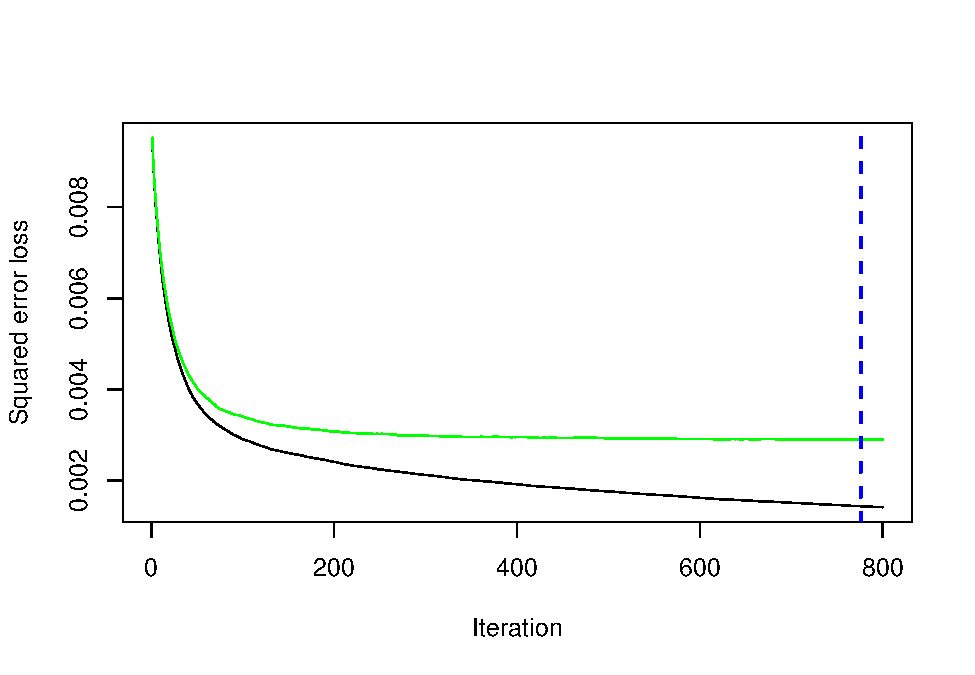
\includegraphics{BiasVarianceTradeoff_files/figure-latex/unnamed-chunk-5-1.pdf}

\begin{Shaded}
\begin{Highlighting}[]
\NormalTok{form0 <-}\StringTok{ "y ~ "}
\NormalTok{f <-}\StringTok{ }\NormalTok{f2}
\KeywordTok{buildGraph}\NormalTok{(}\StringTok{"2"}\NormalTok{)}
\end{Highlighting}
\end{Shaded}

\begin{verbatim}
## [1] "y ~  + I(x^1)"
## [1] 3.481511806 0.110822600 0.002289397 3.062500000
## [1] "y ~  + I(x^1) + I(x^2)"
## [1] 2.9761574567 0.1390961194 0.0006021532 3.0625000000
## [1] "y ~  + I(x^1) + I(x^2) + I(x^3)"
## [1] 3.15324456 0.20231546 0.01196726 3.06250000
## [1] "y ~  + I(x^1) + I(x^2) + I(x^3) + I(x^4)"
## [1] 3.103995981 0.272256804 0.002591607 3.062500000
## [1] "y ~  + I(x^1) + I(x^2) + I(x^3) + I(x^4) + I(x^5)"
## [1] 3.30816993 0.31732962 0.08523738 3.06250000
## [1] "y ~  + I(x^1) + I(x^2) + I(x^3) + I(x^4) + I(x^5) + I(x^6)"
## [1] 3.12580324 0.39764898 0.01478932 3.06250000
## [1] "y ~  + I(x^1) + I(x^2) + I(x^3) + I(x^4) + I(x^5) + I(x^6) + I(x^7)"
## [1] 3.58568399 0.40383022 0.01482348 3.06250000
## [1] "y ~  + I(x^1) + I(x^2) + I(x^3) + I(x^4) + I(x^5) + I(x^6) + I(x^7) + I(x^8)"
## [1] 3.673956498 0.437909149 0.001615856 3.062500000
## [1] "y ~  + I(x^1) + I(x^2) + I(x^3) + I(x^4) + I(x^5) + I(x^6) + I(x^7) + I(x^8) + I(x^9)"
## [1] 3.882051286 0.484099121 0.003647821 3.062500000
## [1] "y ~  + I(x^1) + I(x^2) + I(x^3) + I(x^4) + I(x^5) + I(x^6) + I(x^7) + I(x^8) + I(x^9) + I(x^10)"
## [1] 3.4912987882 0.6273891172 0.0002876566 3.0625000000
## [1] "y ~  + I(x^1) + I(x^2) + I(x^3) + I(x^4) + I(x^5) + I(x^6) + I(x^7) + I(x^8) + I(x^9) + I(x^10) + I(x^11)"
## [1] 4.0024252133 0.8996105979 0.0006017353 3.0625000000
## [1] "y ~  + I(x^1) + I(x^2) + I(x^3) + I(x^4) + I(x^5) + I(x^6) + I(x^7) + I(x^8) + I(x^9) + I(x^10) + I(x^11) + I(x^12)"
## [1] 3.897761517 0.971422618 0.009300845 3.062500000
## [1] "y ~  + I(x^1) + I(x^2) + I(x^3) + I(x^4) + I(x^5) + I(x^6) + I(x^7) + I(x^8) + I(x^9) + I(x^10) + I(x^11) + I(x^12) + I(x^13)"
## [1] 4.2249130774 0.9149092916 0.0005067525 3.0625000000
## [1] "y ~  + I(x^1) + I(x^2) + I(x^3) + I(x^4) + I(x^5) + I(x^6) + I(x^7) + I(x^8) + I(x^9) + I(x^10) + I(x^11) + I(x^12) + I(x^13) + I(x^14)"
## [1] 4.1719314 0.8400855 0.0111516 3.0625000
## [1] "y ~  + I(x^1) + I(x^2) + I(x^3) + I(x^4) + I(x^5) + I(x^6) + I(x^7) + I(x^8) + I(x^9) + I(x^10) + I(x^11) + I(x^12) + I(x^13) + I(x^14) + I(x^15)"
## [1] 3.8101141100 1.0384747024 0.0005673913 3.0625000000
\end{verbatim}

\includegraphics{BiasVarianceTradeoff_files/figure-latex/unnamed-chunk-5-2.pdf}

\begin{Shaded}
\begin{Highlighting}[]
\NormalTok{form0 <-}\StringTok{ "y ~ "}
\NormalTok{f <-}\StringTok{ }\NormalTok{f3}
\KeywordTok{buildGraph}\NormalTok{(}\StringTok{"3"}\NormalTok{)}
\end{Highlighting}
\end{Shaded}

\begin{verbatim}
## [1] "y ~  + I(x^1)"
## [1] 3.22039070 0.12185849 0.02947788 3.06250000
## [1] "y ~  + I(x^1) + I(x^2)"
## [1] 3.318137212 0.132661469 0.005368728 3.062500000
## [1] "y ~  + I(x^1) + I(x^2) + I(x^3)"
## [1] 3.467933333 0.206526486 0.007591408 3.062500000
## [1] "y ~  + I(x^1) + I(x^2) + I(x^3) + I(x^4)"
## [1] 3.405636667 0.282435819 0.001159452 3.062500000
## [1] "y ~  + I(x^1) + I(x^2) + I(x^3) + I(x^4) + I(x^5)"
## [1] 3.422061643 0.265905299 0.001605231 3.062500000
## [1] "y ~  + I(x^1) + I(x^2) + I(x^3) + I(x^4) + I(x^5) + I(x^6)"
## [1] 3.635791557 0.331664225 0.004750779 3.062500000
## [1] "y ~  + I(x^1) + I(x^2) + I(x^3) + I(x^4) + I(x^5) + I(x^6) + I(x^7)"
## [1] 3.489408032 0.387232325 0.001640798 3.062500000
## [1] "y ~  + I(x^1) + I(x^2) + I(x^3) + I(x^4) + I(x^5) + I(x^6) + I(x^7) + I(x^8)"
## [1] 3.704480928 0.444777552 0.001703175 3.062500000
## [1] "y ~  + I(x^1) + I(x^2) + I(x^3) + I(x^4) + I(x^5) + I(x^6) + I(x^7) + I(x^8) + I(x^9)"
## [1] 4.02101131 0.54276529 0.01587562 3.06250000
## [1] "y ~  + I(x^1) + I(x^2) + I(x^3) + I(x^4) + I(x^5) + I(x^6) + I(x^7) + I(x^8) + I(x^9) + I(x^10)"
## [1] 3.2621288 0.6000962 0.0209090 3.0625000
## [1] "y ~  + I(x^1) + I(x^2) + I(x^3) + I(x^4) + I(x^5) + I(x^6) + I(x^7) + I(x^8) + I(x^9) + I(x^10) + I(x^11)"
## [1] 4.075184818 0.646123350 0.001657847 3.062500000
## [1] "y ~  + I(x^1) + I(x^2) + I(x^3) + I(x^4) + I(x^5) + I(x^6) + I(x^7) + I(x^8) + I(x^9) + I(x^10) + I(x^11) + I(x^12)"
## [1] 4.28149638 0.90919673 0.02813572 3.06250000
## [1] "y ~  + I(x^1) + I(x^2) + I(x^3) + I(x^4) + I(x^5) + I(x^6) + I(x^7) + I(x^8) + I(x^9) + I(x^10) + I(x^11) + I(x^12) + I(x^13)"
## [1] 4.037847538 0.950281011 0.004842282 3.062500000
## [1] "y ~  + I(x^1) + I(x^2) + I(x^3) + I(x^4) + I(x^5) + I(x^6) + I(x^7) + I(x^8) + I(x^9) + I(x^10) + I(x^11) + I(x^12) + I(x^13) + I(x^14)"
## [1] 4.40909723 0.95849264 0.01062642 3.06250000
## [1] "y ~  + I(x^1) + I(x^2) + I(x^3) + I(x^4) + I(x^5) + I(x^6) + I(x^7) + I(x^8) + I(x^9) + I(x^10) + I(x^11) + I(x^12) + I(x^13) + I(x^14) + I(x^15)"
## [1] 4.148622364 1.056968094 0.000751375 3.062500000
\end{verbatim}

\includegraphics{BiasVarianceTradeoff_files/figure-latex/unnamed-chunk-5-3.pdf}

\begin{Shaded}
\begin{Highlighting}[]
\NormalTok{form0 <-}\StringTok{ "y ~ "}
\NormalTok{f <-}\StringTok{ }\NormalTok{f4}
\KeywordTok{buildGraph}\NormalTok{(}\StringTok{"4"}\NormalTok{)}
\end{Highlighting}
\end{Shaded}

\begin{verbatim}
## [1] "y ~  + I(x^1)"
## [1] 3.265142621 0.127111786 0.002785524 3.062500000
## [1] "y ~  + I(x^1) + I(x^2)"
## [1] 2.903587342 0.121779791 0.002244499 3.062500000
## [1] "y ~  + I(x^1) + I(x^2) + I(x^3)"
## [1] 3.31746160 0.17471910 0.06142804 3.06250000
## [1] "y ~  + I(x^1) + I(x^2) + I(x^3) + I(x^4)"
## [1] 3.4888631275 0.2725921177 0.0001091888 3.0625000000
## [1] "y ~  + I(x^1) + I(x^2) + I(x^3) + I(x^4) + I(x^5)"
## [1] 3.317304315 0.303666622 0.001085139 3.062500000
## [1] "y ~  + I(x^1) + I(x^2) + I(x^3) + I(x^4) + I(x^5) + I(x^6)"
## [1] 2.975246435 0.318536203 0.001881754 3.062500000
## [1] "y ~  + I(x^1) + I(x^2) + I(x^3) + I(x^4) + I(x^5) + I(x^6) + I(x^7)"
## [1] 3.460880e+00 4.987964e-01 2.130372e-05 3.062500e+00
## [1] "y ~  + I(x^1) + I(x^2) + I(x^3) + I(x^4) + I(x^5) + I(x^6) + I(x^7) + I(x^8)"
## [1] 3.224021575 0.455289641 0.004385677 3.062500000
## [1] "y ~  + I(x^1) + I(x^2) + I(x^3) + I(x^4) + I(x^5) + I(x^6) + I(x^7) + I(x^8) + I(x^9)"
## [1] 3.673858306 0.618114443 0.003905766 3.062500000
## [1] "y ~  + I(x^1) + I(x^2) + I(x^3) + I(x^4) + I(x^5) + I(x^6) + I(x^7) + I(x^8) + I(x^9) + I(x^10)"
## [1] 3.615592534 0.587404553 0.009833623 3.062500000
## [1] "y ~  + I(x^1) + I(x^2) + I(x^3) + I(x^4) + I(x^5) + I(x^6) + I(x^7) + I(x^8) + I(x^9) + I(x^10) + I(x^11)"
## [1] 3.8646159 0.7235673 0.0274561 3.0625000
## [1] "y ~  + I(x^1) + I(x^2) + I(x^3) + I(x^4) + I(x^5) + I(x^6) + I(x^7) + I(x^8) + I(x^9) + I(x^10) + I(x^11) + I(x^12)"
## [1] 4.120928550 0.918583079 0.005820165 3.062500000
## [1] "y ~  + I(x^1) + I(x^2) + I(x^3) + I(x^4) + I(x^5) + I(x^6) + I(x^7) + I(x^8) + I(x^9) + I(x^10) + I(x^11) + I(x^12) + I(x^13)"
## [1] 3.839701e+00 8.772512e-01 8.711797e-05 3.062500e+00
## [1] "y ~  + I(x^1) + I(x^2) + I(x^3) + I(x^4) + I(x^5) + I(x^6) + I(x^7) + I(x^8) + I(x^9) + I(x^10) + I(x^11) + I(x^12) + I(x^13) + I(x^14)"
## [1] 4.249237416 1.043943261 0.003759531 3.062500000
## [1] "y ~  + I(x^1) + I(x^2) + I(x^3) + I(x^4) + I(x^5) + I(x^6) + I(x^7) + I(x^8) + I(x^9) + I(x^10) + I(x^11) + I(x^12) + I(x^13) + I(x^14) + I(x^15)"
## [1] 3.83118275 1.24218864 0.01310362 3.06250000
\end{verbatim}

\includegraphics{BiasVarianceTradeoff_files/figure-latex/unnamed-chunk-5-4.pdf}

\hypertarget{assignment-2}{%
\subsection{Assignment 2}\label{assignment-2}}

\begin{Shaded}
\begin{Highlighting}[]
\NormalTok{maxK <-}\StringTok{ }\DecValTok{20}
\NormalTok{f <-}\StringTok{ }\NormalTok{f1}
\KeywordTok{buildGraph.knn}\NormalTok{(}\StringTok{"1"}\NormalTok{)}
\end{Highlighting}
\end{Shaded}

\begin{verbatim}
## [1] "K=3"
## [1] 3.74090184 0.98210122 0.01215996 3.06250000
## [1] "K=4"
## [1] 3.8786385438 0.7709503253 0.0004468776 3.0625000000
## [1] "K=5"
## [1] 3.27296896 0.60168552 0.01070029 3.06250000
## [1] "K=6"
## [1] 3.782860e+00 4.794410e-01 9.629507e-06 3.062500e+00
## [1] "K=7"
## [1] 3.631028766 0.402388254 0.007995343 3.062500000
## [1] "K=8"
## [1] 2.827425512 0.334349473 0.003697477 3.062500000
## [1] "K=9"
## [1] 3.35639176 0.36292916 0.02244452 3.06250000
## [1] "K=10"
## [1] 3.535486013 0.306940708 0.003265348 3.062500000
## [1] "K=11"
## [1] 3.180236752 0.277991022 0.009362964 3.062500000
## [1] "K=12"
## [1] 3.459669744 0.254330198 0.002436295 3.062500000
## [1] "K=13"
## [1] 3.65102995 0.24786131 0.02595039 3.06250000
## [1] "K=14"
## [1] 3.09997843 0.21089382 0.02615714 3.06250000
## [1] "K=15"
## [1] 3.457990957 0.216991751 0.005463764 3.062500000
## [1] "K=16"
## [1] 3.39679577 0.20210732 0.02502078 3.06250000
## [1] "K=17"
## [1] 3.1831405683 0.1806272531 0.0000361634 3.0625000000
## [1] "K=18"
## [1] 3.012767158 0.180768193 0.001129928 3.062500000
## [1] "K=19"
## [1] 3.13906125 0.18074209 0.01056385 3.06250000
## [1] "K=20"
## [1] 3.23134785 0.14886597 0.03716801 3.06250000
\end{verbatim}

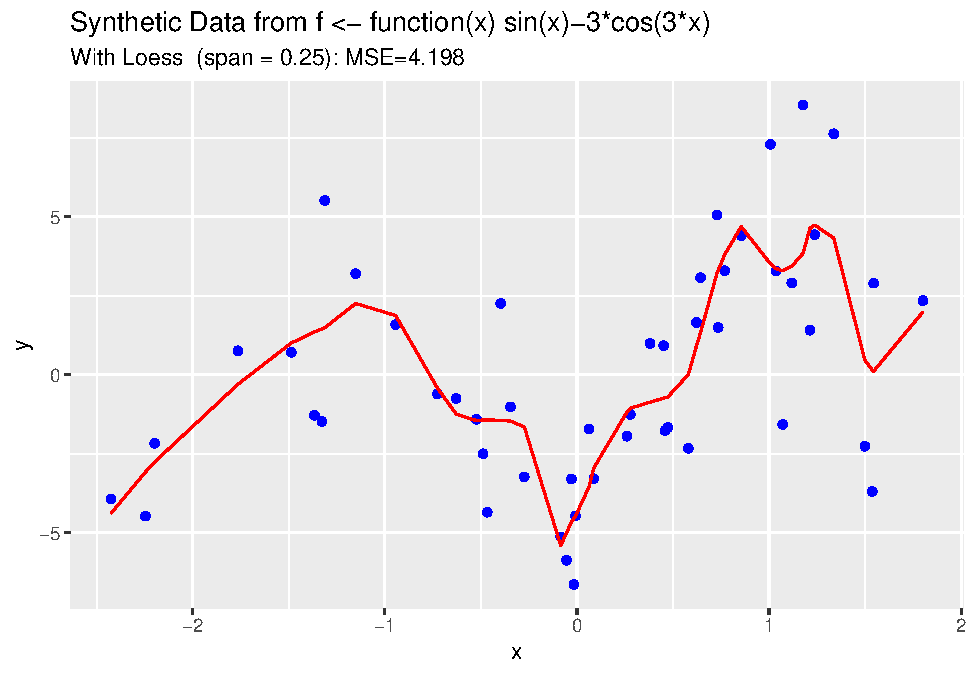
\includegraphics{BiasVarianceTradeoff_files/figure-latex/unnamed-chunk-6-1.pdf}

\begin{Shaded}
\begin{Highlighting}[]
\NormalTok{f <-}\StringTok{ }\NormalTok{f2}
\KeywordTok{buildGraph.knn}\NormalTok{(}\StringTok{"2"}\NormalTok{)}
\end{Highlighting}
\end{Shaded}

\begin{verbatim}
## [1] "K=3"
## [1] 3.7755178859 1.0180751643 0.0001400284 3.0625000000
## [1] "K=4"
## [1] 4.0843930865 0.8392090100 0.0003402748 3.0625000000
## [1] "K=5"
## [1] 3.7795598920 0.4683849913 0.0001501272 3.0625000000
## [1] "K=6"
## [1] 3.365689895 0.488244433 0.001239273 3.062500000
## [1] "K=7"
## [1] 3.603259602 0.388236668 0.002057591 3.062500000
## [1] "K=8"
## [1] 3.18276664 0.41596979 0.01561779 3.06250000
## [1] "K=9"
## [1] 3.2470732796 0.3298515749 0.0009265501 3.0625000000
## [1] "K=10"
## [1] 3.013086186 0.317641648 0.002947568 3.062500000
## [1] "K=11"
## [1] 3.325866036 0.294585018 0.005833047 3.062500000
## [1] "K=12"
## [1] 3.26121495 0.24544163 0.02592738 3.06250000
## [1] "K=13"
## [1] 3.565056255 0.244202623 0.002240142 3.062500000
## [1] "K=14"
## [1] 3.08059728 0.21018022 0.02093072 3.06250000
## [1] "K=15"
## [1] 3.195506064 0.221812693 0.003576656 3.062500000
## [1] "K=16"
## [1] 3.641610650 0.178555206 0.001948563 3.062500000
## [1] "K=17"
## [1] 3.04706405 0.18803179 0.02431563 3.06250000
## [1] "K=18"
## [1] 3.6041199129 0.1807917188 0.0006350071 3.0625000000
## [1] "K=19"
## [1] 3.028521e+00 1.709698e-01 2.877947e-07 3.062500e+00
## [1] "K=20"
## [1] 3.08090069 0.16311355 0.01001875 3.06250000
\end{verbatim}

\includegraphics{BiasVarianceTradeoff_files/figure-latex/unnamed-chunk-6-2.pdf}

\begin{Shaded}
\begin{Highlighting}[]
\NormalTok{f <-}\StringTok{ }\NormalTok{f3}
\KeywordTok{buildGraph.knn}\NormalTok{(}\StringTok{"3"}\NormalTok{)}
\end{Highlighting}
\end{Shaded}

\begin{verbatim}
## [1] "K=3"
## [1] 4.041783359 1.009894348 0.002123416 3.062500000
## [1] "K=4"
## [1] 3.4960516429 0.6663825268 0.0006250751 3.0625000000
## [1] "K=5"
## [1] 3.9330770719 0.5793985744 0.0003158133 3.0625000000
## [1] "K=6"
## [1] 3.2740365135 0.4762546894 0.0002238754 3.0625000000
## [1] "K=7"
## [1] 3.23303422 0.41258061 0.00348466 3.06250000
## [1] "K=8"
## [1] 3.382014e+00 3.990942e-01 5.191829e-05 3.062500e+00
## [1] "K=9"
## [1] 3.471892573 0.320411338 0.004859532 3.062500000
## [1] "K=10"
## [1] 3.444975e+00 3.256558e-01 1.206328e-05 3.062500e+00
## [1] "K=11"
## [1] 3.53592308 0.33074341 0.02176743 3.06250000
## [1] "K=12"
## [1] 3.348240770 0.239926182 0.005338103 3.062500000
## [1] "K=13"
## [1] 3.4717220273 0.2592979704 0.0001698339 3.0625000000
## [1] "K=14"
## [1] 3.412705592 0.198235261 0.001337682 3.062500000
## [1] "K=15"
## [1] 2.915601154 0.206260043 0.002786636 3.062500000
## [1] "K=16"
## [1] 3.174455783 0.206708224 0.001502876 3.062500000
## [1] "K=17"
## [1] 3.492540214 0.181822173 0.002833284 3.062500000
## [1] "K=18"
## [1] 3.2768185325 0.1561636799 0.0008093766 3.0625000000
## [1] "K=19"
## [1] 3.38544810 0.17400144 0.02705182 3.06250000
## [1] "K=20"
## [1] 3.039290e+00 1.625360e-01 9.229829e-05 3.062500e+00
\end{verbatim}

\includegraphics{BiasVarianceTradeoff_files/figure-latex/unnamed-chunk-6-3.pdf}

\begin{Shaded}
\begin{Highlighting}[]
\NormalTok{f <-}\StringTok{ }\NormalTok{f4}
\KeywordTok{buildGraph.knn}\NormalTok{(}\StringTok{"4"}\NormalTok{)}
\end{Highlighting}
\end{Shaded}

\begin{verbatim}
## [1] "K=3"
## [1] 4.204925125 0.942503760 0.006332675 3.062500000
## [1] "K=4"
## [1] 3.62901570 0.77508143 0.03309072 3.06250000
## [1] "K=5"
## [1] 3.40700551 0.61602079 0.03069945 3.06250000
## [1] "K=6"
## [1] 3.80340372 0.54988760 0.01874738 3.06250000
## [1] "K=7"
## [1] 3.41141010 0.45740046 0.01354214 3.06250000
## [1] "K=8"
## [1] 3.87967859 0.38767278 0.00913799 3.06250000
## [1] "K=9"
## [1] 3.49644834 0.34372084 0.02507925 3.06250000
## [1] "K=10"
## [1] 3.4368662818 0.3430547244 0.0004010764 3.0625000000
## [1] "K=11"
## [1] 3.46337970 0.27102075 0.01590297 3.06250000
## [1] "K=12"
## [1] 3.325568077 0.250632473 0.009448769 3.062500000
## [1] "K=13"
## [1] 3.54264570 0.26211260 0.01187698 3.06250000
## [1] "K=14"
## [1] 3.06987436 0.21421977 0.02496539 3.06250000
## [1] "K=15"
## [1] 3.06352014 0.19006563 0.01611078 3.06250000
## [1] "K=16"
## [1] 2.969287e+00 2.056641e-01 7.516014e-05 3.062500e+00
## [1] "K=17"
## [1] 3.3957811128 0.1634522400 0.0002428576 3.0625000000
## [1] "K=18"
## [1] 3.334015004 0.176865775 0.002502463 3.062500000
## [1] "K=19"
## [1] 3.095609253 0.175157485 0.001167175 3.062500000
## [1] "K=20"
## [1] 3.2016199714 0.1646103749 0.0000855826 3.0625000000
\end{verbatim}

\includegraphics{BiasVarianceTradeoff_files/figure-latex/unnamed-chunk-6-4.pdf}

\end{document}
